\section{Flyweight}

O padrão Flyweight permite economizar o espaço em memória 
da aplicação ao fornecer uma instância compartilhada de 
uma classe para que ela não precise ser instanciada 
mais de uma vez. A Figura \ref{flyweight_struct} mostra 
a estrutura do padrão. Nela, uma interface Flyweight 
define um elemento reutilizável, sendo implementada 
pelas classes ConcreteFlyweight e UnsharedConcreteFlyweight. 
A classe ConcreteFlyweight armazena um estado intrínseco 
e define uma operação que depende de um estado extrínseco 
para ser executada. \cite{gamma:1995}

Duas classes merecem atenção nesse diagrama. A primeira 
é a FlyweightFactory. Essa classe é adicionada para 
gerenciar a criação dos Flyweights e garantir que as 
instâncias da classe serão reutilizadas. Ela armazena, em 
seus atributos, uma lista de objetos Flyweight para que,  
quando solicitada pelo cliente, seja verificado se a instância 
desejada já existe. Caso não exista, ela é criada e 
adicionada à lista. 

A segunda classe que merece atenção é a UnsharedConcreteFlyweight, 
que é necessária caso existam elementos específicos 
do tipo Flyweight que não possam ser compartilhados. 
Esses elementos não podem ser criados através da 
FlyweightFactory.

\begin{figure}[htb]
	\caption{\label{flyweight_struct}Estrutura do Flyweight.}
	\begin{center}
	    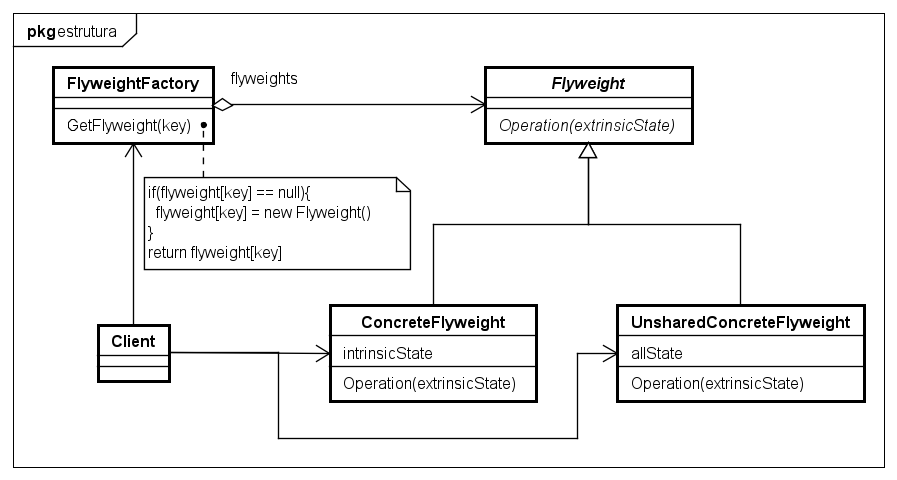
\includegraphics[scale=0.5]{5_padroes-contexto-funcional/5.2_estruturais/5.2.6_flyweight/flyweight_estrutura.png}
	\end{center}
\end{figure}

\subsection*{Exemplo Orientado a Objetos}

Um editor de documentos possui uma ferramenta 
de formatação e edição de textos. Para reduzir o 
custo de memória, as classes que armazenam os 
caracteres do alfabeto devem ser compartilhadas, 
dada a quantidade de instâncias de um mesmo caracter 
que existiriam em um texto com milhares de palavras. 
Ao mesmo tempo, a ferramenta deve armazenar dois 
elementos que não podem ser compartilhados com as 
letras - a linha e a coluna onde cada letra está 
localizada. 

A Figura \ref{flyweight_exemplo} apresenta o diagrama 
de classes para esse exemplo. A interface Glyph 
representa um elemento textual. As classes Row e 
Column armazenam em seus atributos um conjunto de objetos 
do tipo Glyph. 
Por fim, a classe Character armazena em seus atributos 
o caracter que deve ser compartilhado. Apenas uma 
instância é criada para cada caracter. O 
Código \ref{ooflyweight} demonstra a implementação 
desse exemplo.

\begin{figure}[htb]
	\caption{\label{flyweight_exemplo}Exemplo de Flyweight.}
	\begin{center}
	    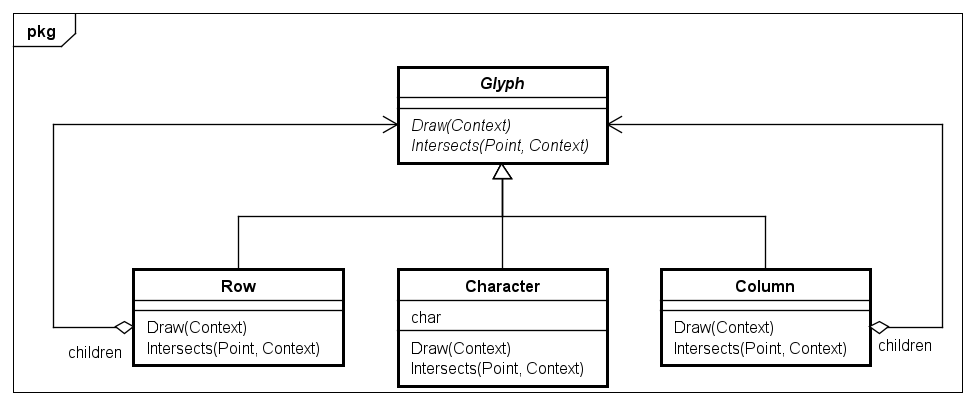
\includegraphics[scale=0.5]{5_padroes-contexto-funcional/5.2_estruturais/5.2.6_flyweight/flyweight_exemplo.png}
	\end{center}
\end{figure}

\begin{lstlisting}[caption={Flyweight Orientado a Objetos.},label=ooflyweight]

trait Glyph {
  def Draw(context : Context)
  def Intersects(point : Point, context : Context)
}

class Character(val character: Char) extends Glyph {
  def Draw(context: Context): Unit = {
    //Desenha o caracter
  }

  def Intersects(point: Point, context: Context): Unit = {
    //Verifica a interseção com o ponto
  }
}

class Row(var children : List[Glyph]) extends Glyph {
  def Draw(context: Context): Unit = {
    //Desenha a linha
  }

  def Intersects(point: Point, context: Context): Unit = {
    //Verifica a interseção com o ponto
  }
}

class Column(var children : List[Glyph]) extends Glyph {
  def Draw(context: Context) : Unit = {
    //Desenha a coluna
  }

  def Intersects(point: Point, context: Context): Unit = {
    //Verifica a interseção com o ponto
  }
}

\end{lstlisting}

\subsection*{Contexto Funcional}

Esse padrão utiliza uma técnica também conhecida 
como memoização, que salva computações já realizadas 
para serem reutilizadas e economizar espaço em 
memória\cite{scalafunctpatterns}. O Código \ref{fpflyweight} 
demonstra como o exemplo anterior poderia ser 
implementado. O tipo GlyphFactory, definido na 
linha 3, é um dicionário cuja chave é do tipo 
String e o valor é do tipo Glyph. A função 
GetGlyph recebe como parâmetro um valor de um 
Glyph e uma fábrica de Glyphs. A função verifica 
se o valor já está contido nos Glyphs criados, 
retornando-o caso exista e criando um novo 
caso não. A desvantagem dessa abordagem é que 
por a função GetGlyph ser pura, é necessário 
sempre receber e retornar o \textit{factory} 
atualizado.

\begin{lstlisting}[caption={Flyweight Funcional.},label=fpflyweight]
    
type Glyph
type GlyphFactory = Map[String, Glyph]

def GetGlyph(value : String, factory : GlyphFactory)
  : (Glyph, GlyphFactory) = {
  factory.get(value) match {
    case Some(glyph) => (glyph, factory)
    case None => {
      val newGlyph = // Cria novo glyph 
      (newGlyph, factory + (value -> newGlyph))
    }
  }
}
    
\end{lstlisting}